\chapter{文獻回顧}







本研究所探討情境下的量測方法有以下需求:有易於拆裝的量測單位與被量測單位,能夠快速進行拆裝、靈活應用於不同場域,而安裝完成後即可進行三維相對位置量測。為滿足靈活且易於安裝且能夠應用在不同場域的特性,需要有體積小、能耗低、所需校正步驟少、能夠使用於不同場域等特色。

因此,本章節先定義所謂相對定位,再介紹現有文獻的定位技術與方法,比較優缺點並凸顯「近紅外光定位」的優勢,近而針對本論文著重的「LED與PD以近紅外光波段進行定位」的文獻進行探討,敘述此領域研究現況與困難。







% 重申自己主要的目標:(只有LED-PD近紅外光波段符合的原因)
% 低成本、不需預先了解環境資訊、裝設範圍小、方便架設、速度

\section{相對定位定義}
\label{chp:relative}
% -(利用數學符號描述相對定位問題的定義(軌跡、時間等))
    
    在開始進入文獻探討之前,需先以數學定義何謂本論文所欲量測之「相對定位」。首先,本論文所討論的情境為一量測物針對另一特定目標物進行相對位置的量測,如智慧工廠內的機械手臂欲取得與移動載具之間的相對關係,以利夾取搬運物品至載具上進行運送。
    
    我們將取得相對位置的一方稱為量測者,如案例中的機械手臂;而量測者所欲取得相對位置的特定物體稱為目標物,如案例中的移動載具;兩者皆為剛體。因此,可以將量測者與目標物各自視為兩移動座標系如圖\ref{pic:homo_trans},兩者在空間中各自有位置、旋轉的六個自由度,可以利用齊次座標轉換(Homogeneous Transformation)表示座標系之間的平移與旋轉(式\ref{eqn:homogeneous}),$^{PL}\boldsymbol{H}$表示將LED座標系上的點轉換至PD座標系上的齊次轉換矩陣,而$^{PL}\boldsymbol{T}$與$^{PL}\boldsymbol{Ro}$各自代表平移與旋轉的轉換矩陣,符號可參考符號列表(第\pageref{chp:symbol}頁)。
    
    \begin{figure}[ht]
        \centering
        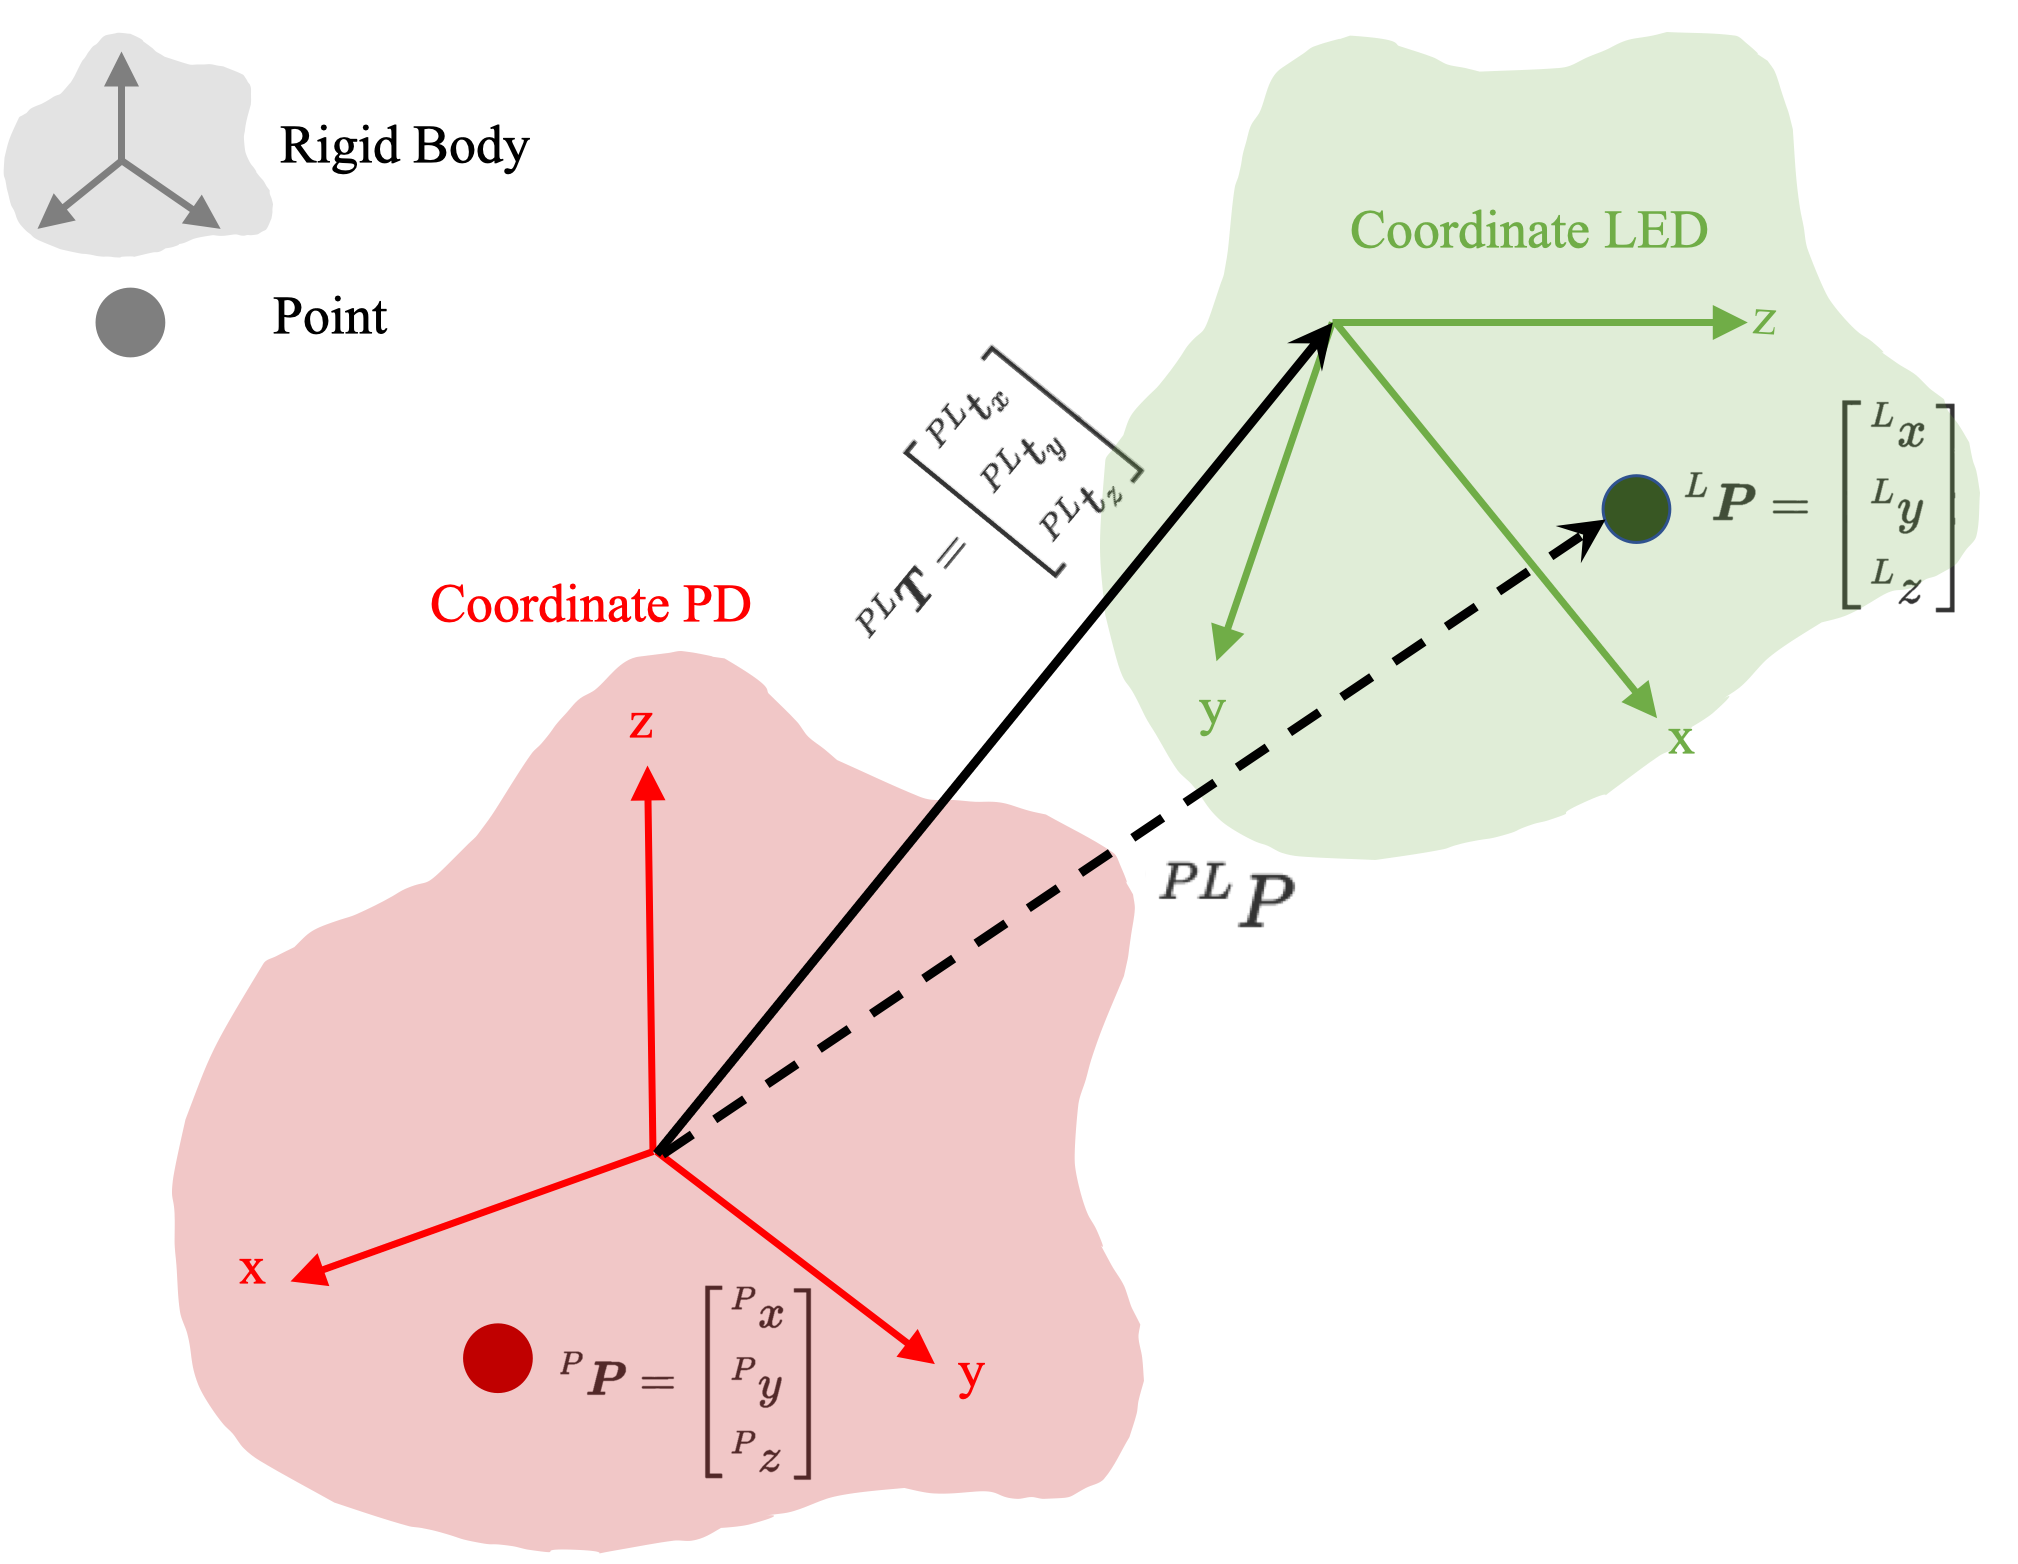
\includegraphics[width=9cm]{ch2pic/homo_trans.png}
        \caption{LED座標系與PD座標系及相對關係}
        \label{pic:homo_trans}
    \end{figure}

    \begin{equation}
        \label{eqn:homogeneous}
        \begin{aligned}
        {\left[\begin{array}{c}
        { }^{P L} P \\
        1
        \end{array}\right]={ }^{P L} \boldsymbol{H}\left[\begin{array}{c}
        { }^{L} P \\
        1
        \end{array}\right] } &=\left[\begin{array}{cc}
        { }^{P L} \boldsymbol{R} \boldsymbol{o} & { }^{P L} \boldsymbol{T} \\
        0 & 1
        \end{array}\right]\left[\begin{array}{c}
        { }^{L} P \\
        1
        \end{array}\right] \\
        &=\left[\begin{array}{cccc}
        { }^{P L} \gamma_{11} & { }^{P L} \gamma_{12} & { }^{P L} \gamma_{13} & { }^{P L} {t}_{x} \\
        { }^{P L} \gamma_{21} & ^{P L } \gamma_{22} & { }^{P L} \gamma_{23} & { }^{P L} {t}_{y} \\
        { }^{P L} \gamma_{31} & ^{P L} \gamma_{32} & { }^{P L} \gamma_{33} & { }^{P L} {t}_{z} \\
        0 & 0 & 0 & 1
        \end{array}\right]\left[\begin{array}{c}
        { }^{L} {x} \\
        { }^{L} {y} \\
        { }^{L} z \\
        1
        \end{array}\right]
        \end{aligned}
    \end{equation}

    % \begin{equation}
    %     ^{PL}\boldsymbol{T}=\left[\begin{array}{l}
    %     ^{PL}x \\ ^{PL}y \\ ^{PL}z
    %     \end{array}\right]
    % \end{equation}

    
    
   其中,兩座標系之間的平移關係$^{PL}\boldsymbol{T}$即為欲得到的相對位置資訊,共有三個自由度。

 



\section{定位方法介紹}
(這段或許可以省略)
    % 補
    - 定位方法介紹:RSS、TDOA這些
    
    % (Ref幾篇Review)
    
    - 先用方法得到角度、距離資訊:利用RSS、TDOA比較
    - 組合角度、距離資訊得到位置:Multitrileration, Fingerprinting

\section{定位技術介紹}

    室內定位所使用的技術(Technique)十分多樣,包含使用電磁波段內的Wifi、藍芽、RFID(Radio Frequency Identification,無線射頻辨識)、可見光定位以及相機定位等,其他使用非電磁波斷的室內定位技術主要為超聲波,應用ToF方法量測訊號發射至接收的時間,然而該技術受溫度影響,且對目標物的辨識能力不佳,目前著重在自駕車與載具中障礙物的有無偵測上\cite{survey_ultrasonic},並不符合研究目標,因此以下章節聚焦在電磁波斷的定位進行分析。

    \subsection{以電磁波頻率切入}

        如讓所述,電磁波段內有許多不同現今受到關注的量測技術,而電磁波以光速傳播,擁有高傳播速度與不受介質溫度與濕度影響的特性,減少可能對量測訊號造成影響的因素。

        本段落由電磁波的頻率切入,頻譜圖如圖\ref{pic:spectrum},大致分為三部分探討:頻率高於790THz的高能量波段、頻率介於790THz與300GHz之間的光波段、頻率低於300GHz的低頻波段\cite{book_electromagnetic}。

        \begin{figure}[ht]
            \centering
            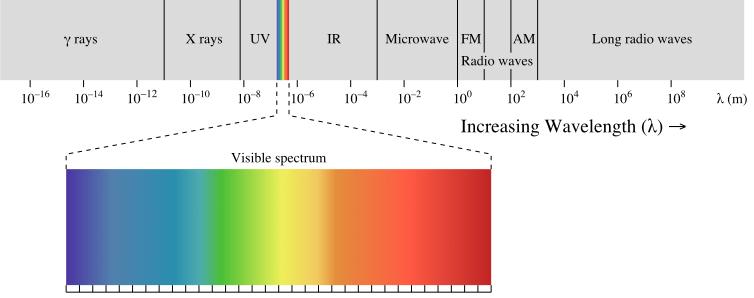
\includegraphics[width=9cm]{ch2pic/electro_spectrum.png}
            \caption{電磁波頻譜度\cite{Spectrum}}
            \label{pic:spectrum}
        \end{figure}
        
        首先,電磁波頻率越高所含能量越高,此特性使得高頻波段(X光、紫外線、伽瑪射線)對人體有害,因此無法使用於定位。
        
        比較光波段與低頻波段的特性:首先,光波段無法穿透障礙物,僅能進行可視範圍內(LoS)的定位;反之低頻波段擁有穿透大多障礙物的特性,因此可用於跨房間、非可視範圍(NLoS)的定位\cite{survey_indoor2018}。非可視範圍定位增加了應用場域,然而也大大提升了訊號處理的難度,感測器難以辨別訊號衰減原因為距離、角度、亦或是障礙物,因此選擇非可視範圍內定位即捨棄精度。舉RFID定位來說,大多應用在固定的場域中建立數據庫,或是利用大量的感測器與訊號發射器來判斷定位\cite{survey_rfid}。

        \begin{figure}[ht]
            \centering
            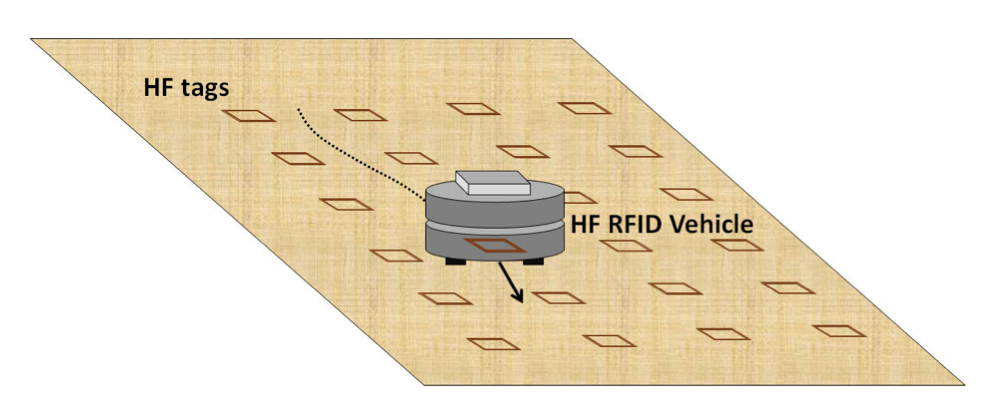
\includegraphics[width=5cm]{ch2pic/rfid_system.png}
            \caption{RFID定位系統示意\cite{survey_rfid}}
            \label{pic:rfid_system}
        \end{figure}

        電磁波另一個特性為:波長愈短可達到的量測精度愈高,且感測器與訊號發射器的硬體大小也愈小,例如市售便宜常見的光波段感測器如PD感光二極體尺寸量級為mm或以下\cite{datasheet:led_sfh4545}且能耗低,而RFID的感測器常見量級為cm\cite{datasheet:rfid_tag}。

        \hspace*{\fill}

        綜上所述,比較低頻波段與光波段,從精度層面來看,光波段捨棄非可視範圍的定位以減少影響訊號的因素,加上波長較短的特性,較符合本研究目標;針對靈活應用的需求,光波段無論是小體積還是低能耗,都是較佳的選擇。因此,根據本研究目標所需,將研究方法聚焦在光波段的定位上。


%_________________________________________
    \subsection{光波段定位}

        
        光波段的定位發展近幾年來十分顯著,主要原因為光學硬體上的進步,促使光通訊(LC, Light Communication)的發展。光通訊吸引了不少研究人員的注目,尤其是可見光波段的通訊,因能搭配室內的照明光源進行系統建制,以上原因帶動與光通訊息息相關的光定位領域,互相提升附加價值。

        \hspace*{\fill}

        光波段的分類可從兩方向切入:使用波段與感測器硬體選擇,以下依序進行探討:

        \subsubsection{使用波段選擇:可見光或紅外光}

        \begin{description}
        \item[研究普及度]\hfill 

        首先,現今室內定位的研究主要著重在可見光的部分\cite{survey_light2018},搭配著室內環境都具有的光源,其優點強調在不對室內環境進行過多改動上即可進行定位量測。然而本研究需能靈活將光源安裝於任意被觀察物上,因此室內充足的可見光光源並不能成為訊號載體,因此雖然可見光波段擁有較多文獻與研究,其並不符合本研究目標,僅能參考方法與眼算法等,所以挑選光波段重點將著重在降低誤差上。

        \item[硬體技術] \hfill 
        
        光波段的光感測器常見的材料有矽(Si)、鍺(Ge)與III或V族元素,價格最便宜的是矽材料,而矽感測器的感光波段約在400-1000nm,也就是可見光與近紅外光(NIR)波段。這也是為什麼普遍對紅外光波段的硬體都有價格昂貴的印象,但凡波長較長的紅外光在硬體材料便需要使用到昂貴的鍺或其他三五族元素\cite{si_pd}。因此,考量到硬體的價格與普遍性,挑選可見光與近紅外光波段較為合適。

        \item[誤差] \hfill 
        
        利用Photodiode定位最大的困難就是要克服其他光所造成的雜訊(Shot Noise),因此在選擇工作波長時,挑選自然環境中強度較低的波段。日常環境中的光源包含太陽光與燈,太陽光可以從圖\ref{pic:solar_spectrum}太陽輻射波譜(Solar Irradiance Spectrum)觀察強度與波長的關係,低谷出現在760nm左右的氧氣吸收帶(Oxygen A-band)、與940nm和1550nm附近被水蒸氣吸收之波段\cite{book:solar_spectrum}。

        \begin{figure}[ht]
            \centering
            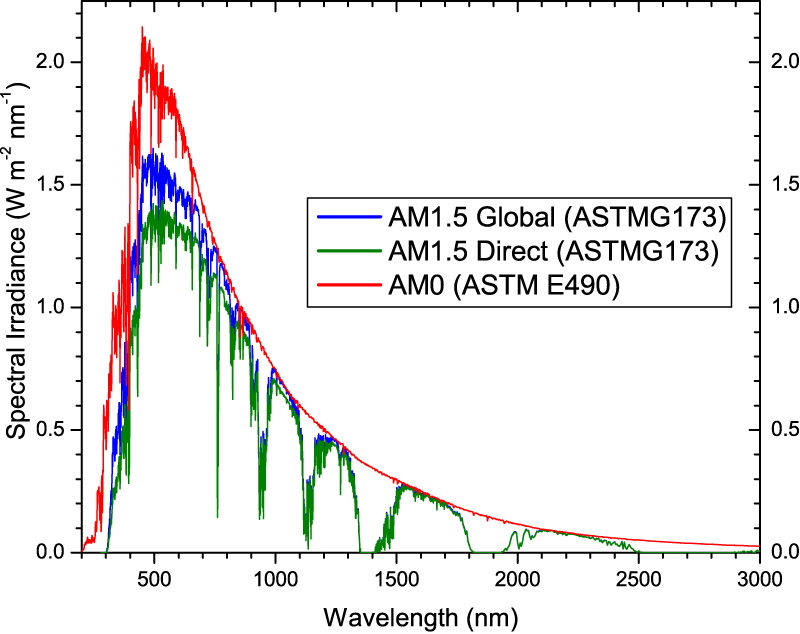
\includegraphics[width=10cm]{ch2pic/solar_spectra.png}
            \caption{太陽輻射波譜\cite{astm}}
            \label{pic:solar_spectrum}
        \end{figure}

        光波段的誤差來源主要包含多重路徑傳輸(Multipath effect)與環境光源(Ambious Light Source),其中環境光強度過高可造成訊號偏移甚至硬體飽和導致訊號失真,因此需有效的降低環境光源的強度以保持定位的準確度。環境光源包含了室內的光源以及太陽光源,室內的光源使用交流電的頻率約在120hz,可以針對頻率進行濾波,而太陽光源的強度則隨頻率增減。從太陽光頻譜圖可以觀察到,太陽光於光波段受到大氣層吸收有三處的能量較低,藉由挑選低谷頻率,即可有效降低太陽光對系統的影響。

        \begin{figure}[ht]
            \centering
            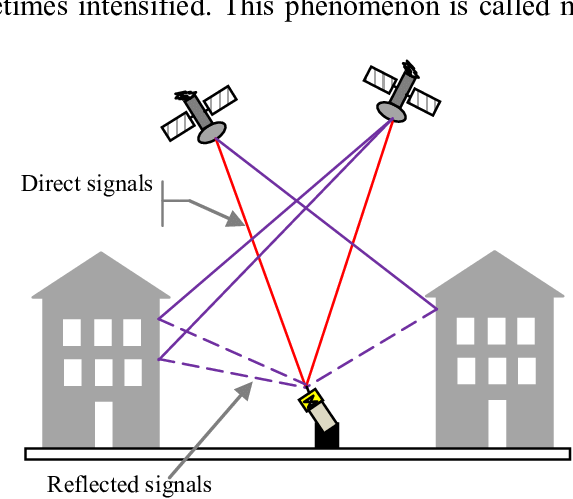
\includegraphics[width=6cm]{ch2pic/multipath.png}
            \caption{多重路徑傳輸\cite{pic:multipath}}
            \label{pic:multipath}
        \end{figure}

        \item[對人眼影響]\hfill 

        本研究目標需應用於移動物體上,因此紅外光呈現優勢,即使光源在環境中的使用者面前直射,紅外光無法在視網膜成像的特性讓使用者並不會感受到影響;反之,朝人眼照射可見光源會造成干擾。除此之外,紅外光頻率低、能量較小,且於視網膜成像的難度也大,因此較為安全。

        \end{description}


        

        \subsubsection{硬體選擇:PD或影像感測器}

            %補


        \subsubsection{小節}
        \hspace*{\fill}
        
        (補圖)
        % [可做一張十字圖:(相機vsPD)(可見光vs紅外光)]

        權衡之下,挑選於太陽光輻射光譜中低谷的760nm與940nm波段,同時享有硬體選擇多且價格低的優勢,又減少了太陽光源所影響的程度,並使裝置保持輕巧低成本又不干擾人眼與日常生活的優點。

\section{LED與PD的定位方法}

    LED與PD的定位方式,是將單個或多個LED安裝在目標物上,各LED藉由編碼來區別各自的訊號,而PD安裝於觀察物上,將每個PD所接收的訊號分別解碼,得到各LED的訊號強度。

    為深入了解系統運作方式,從基本的光領域常用單位切入,開始介紹LED與PD的硬體特性與參數,以及光傳播上的模擬建模,再進入系統整體的細節,以及此領域的文獻探討。

    \subsection{光領域基本介紹}
        
        由於光領域所使用的單位與機械領域差距較大,進入PD與LED定位的探討之前,先對光領域的一些術語與單位進行介紹。

        首先,描述光照的單位在文獻上經常有些混亂,單位分為兩種制度,且常有混用以及口語省略,令人感到困惑,因此以下進行釐清:光領域中的計量單位大致分成兩種系統,輻射測量學(Radiometry)與光度測量學(Photometry),兩領域以不同單位描述光源,其中輻射測量學著重在電磁波輻射的量測,描述通量單位為瓦特(Watt);而光度測量學著重在人演可見之可見光波段的研究,通量單位為流明(Lumen),同樣物理量下單位定義不同。\cite{radiometry_and_photometry}
        

        \begin{figure}[ht]
            \centering
            \caption{輻射測量學與光度測量學的物理量}
            \label{tab:photometry}
            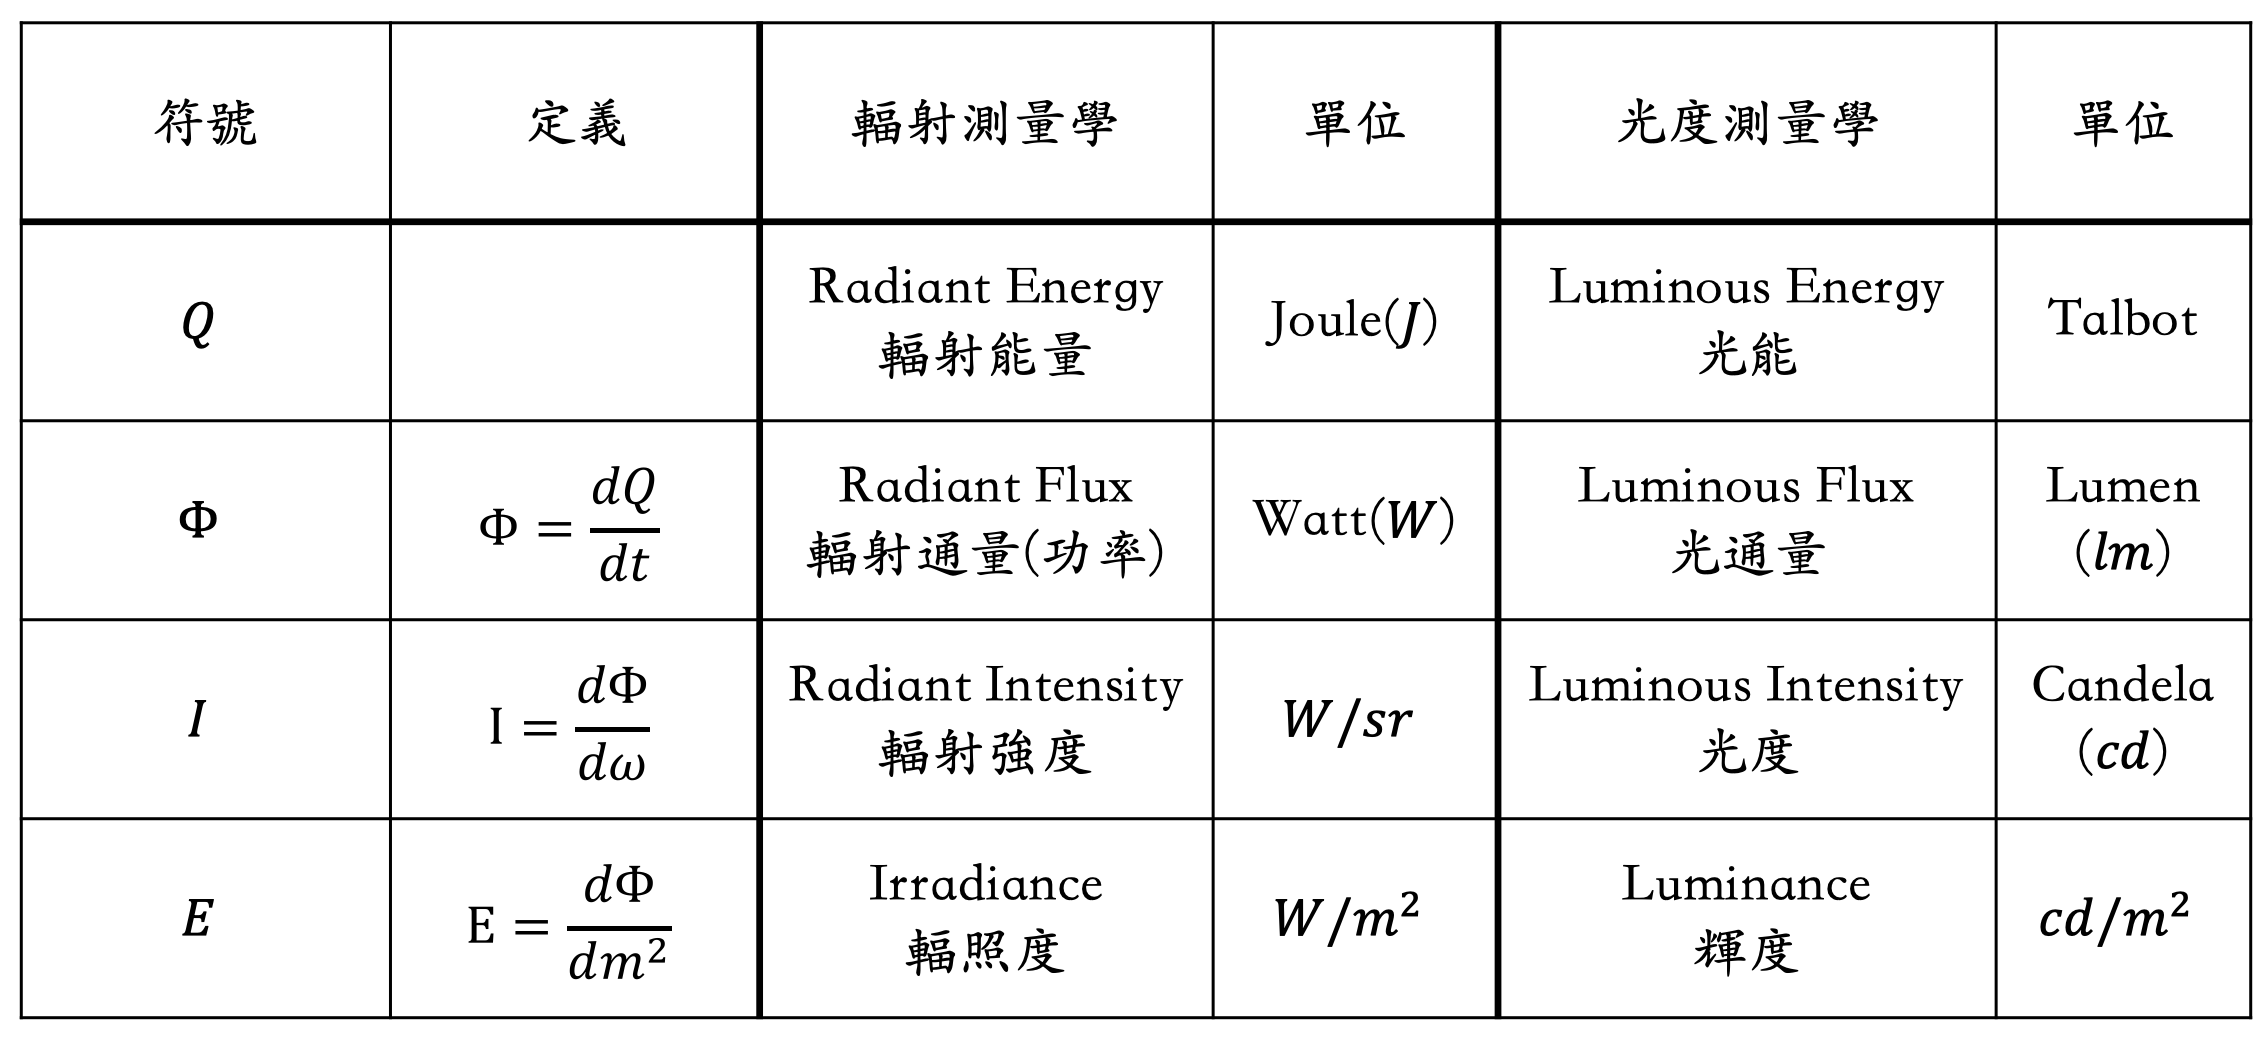
\includegraphics[width=10cm]{ch2pic/photometry_table.png}
        \end{figure}


        本研究聚焦在近紅外光波段,因此本論文所使用的單位系統為輻射測量學的系統,然而文獻上可見光定位數量較多,因此在單位的換算上需特別注意,以下針對光領域常用物理量簡單敘述。

        
        \begin{description}
            \item[立體角 Solid Angle $\Omega$] \hfill
                
                描述二維空間中的角度單位為弧度,表示夾角內的弧長與半徑比例,而單位弧度的定義是半徑與圓弧長度相等時的圓心角。
                然而光源存在於立體空間中,而空間中描述角度的物理量即為立體角(Solid Angle),該物理量代表錐狀立體角在球面上的表面積與半徑平方的比例,其中,單位為球面度(steradians, 簡寫$sr$)代表在半徑為$r$的球體中,立體角投射出的表面積為$r^2$。

                \begin{figure}[ht]
                    \centering
                    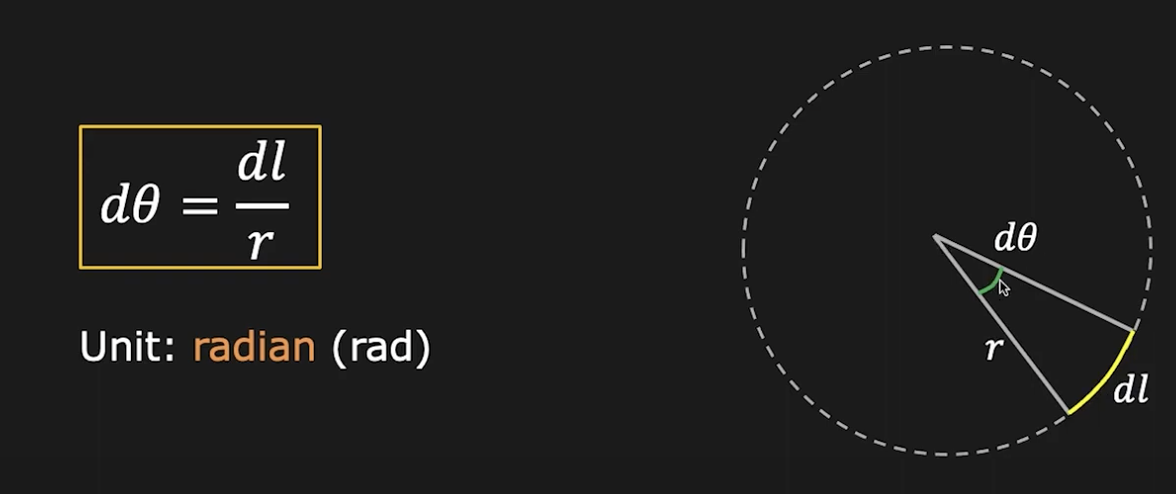
\includegraphics[width=5cm]{00temppic/1.png}
                    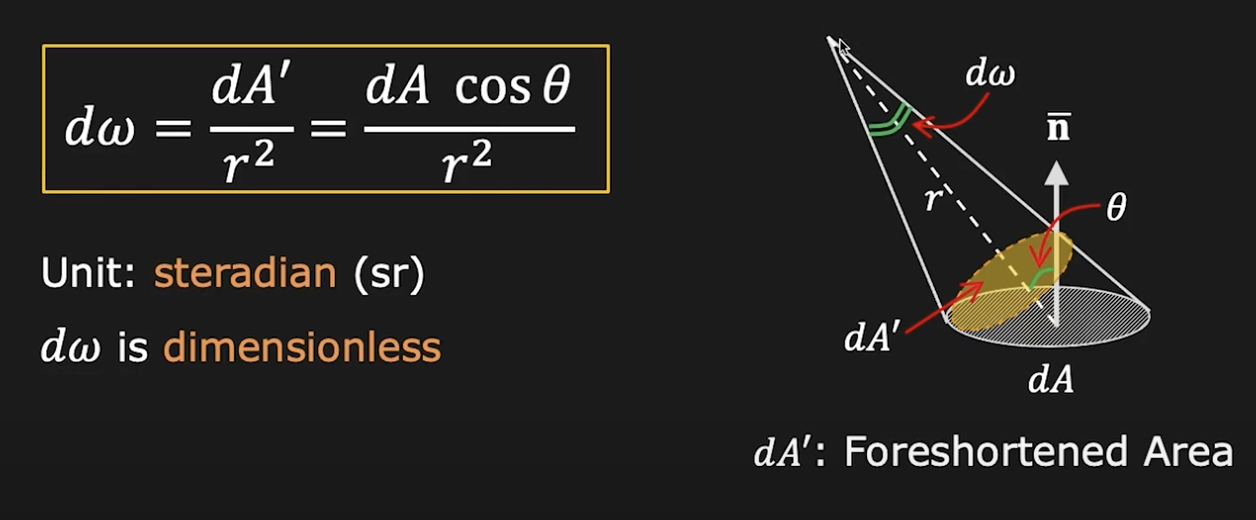
\includegraphics[width=5cm]{00temppic/2.png}
                    % \caption{多重路徑傳輸\cite{pic:multipath}}
                    % \label{pic:multipath}
                \end{figure}

            \item[輻射通量 Radiant Flux $\Phi$]  \hfill
                
                描述光照功率的物理量為通量(Flux)或稱輻射功率(Power),代表每單位時間的輻射能量,單位為瓦特,而大多LED規格表上以此物理量來描述LED在指定電流下可產生的最大光功率。

                \begin{figure}[ht]
                    \centering
                    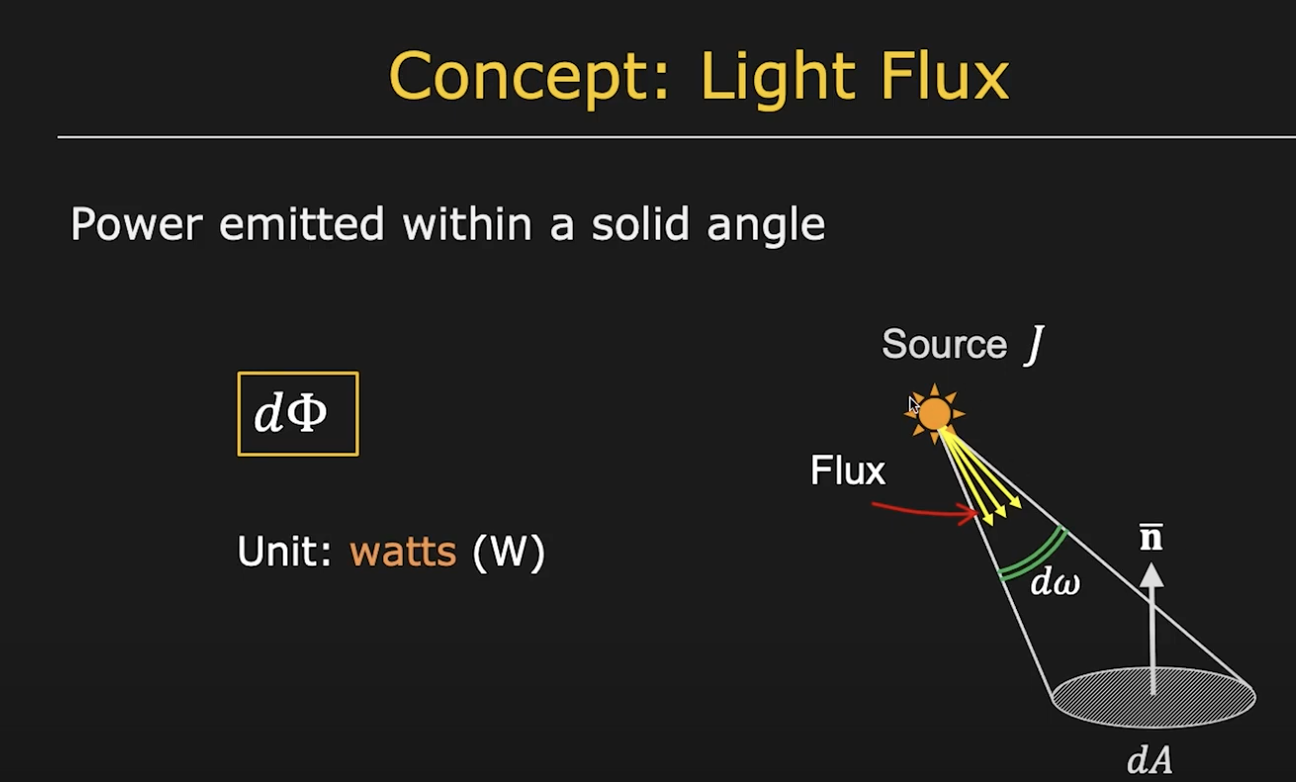
\includegraphics[width=5cm]{00temppic/3.png}
                    % \caption{多重路徑傳輸\cite{pic:multipath}}
                    % \label{pic:multipath}
                \end{figure}

            \item[輻射強度 Radiation Intensity $I$] \hfill
             
                每單位立體角所含的通量稱為輻射強度,此物理量常用於描述光與角度之關係,其與距離無關。
                \begin{figure}[ht]
                    \centering
                    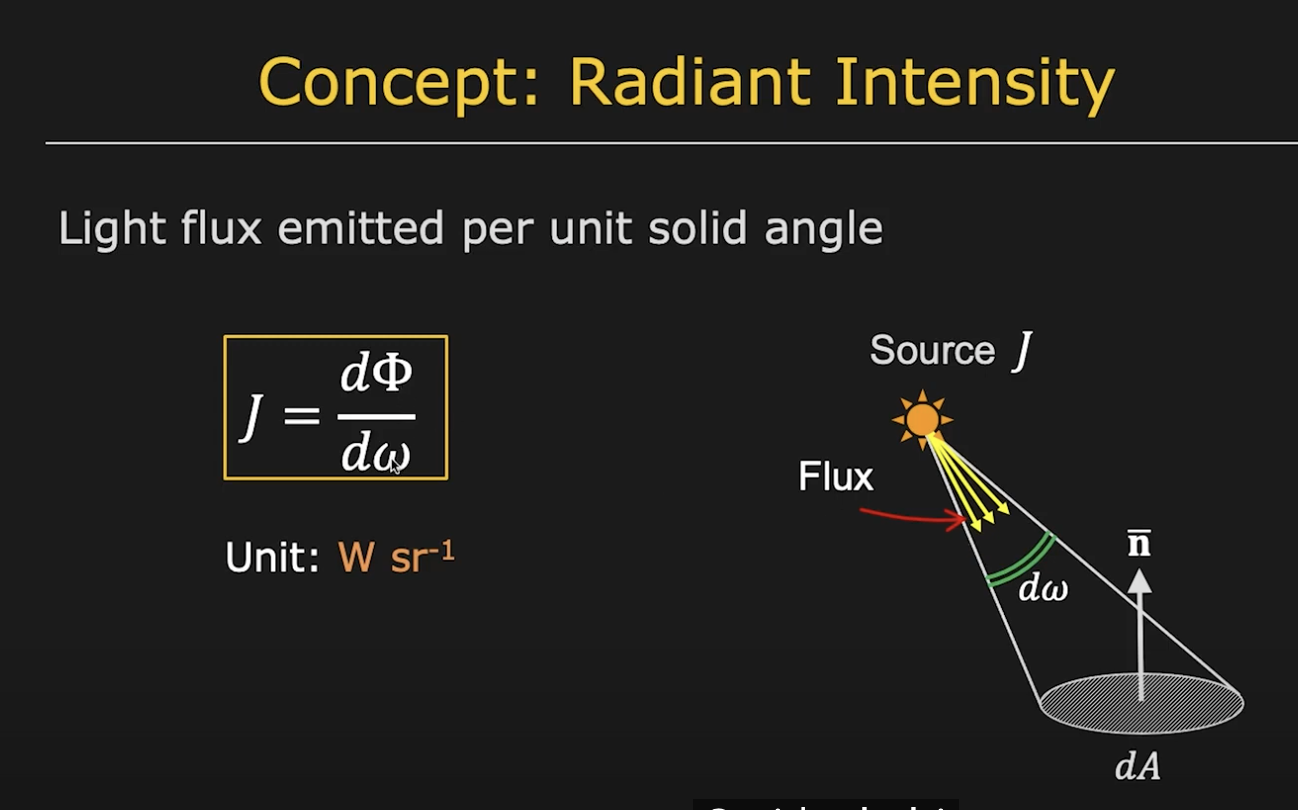
\includegraphics[width=5cm]{00temppic/4.png}
                    % \caption{多重路徑傳輸\cite{pic:multipath}}
                    % \label{pic:multipath}
                \end{figure}

            \item[輻照度 Irradiance $E$] \hfill
                \begin{figure}[ht]
                    \centering
                    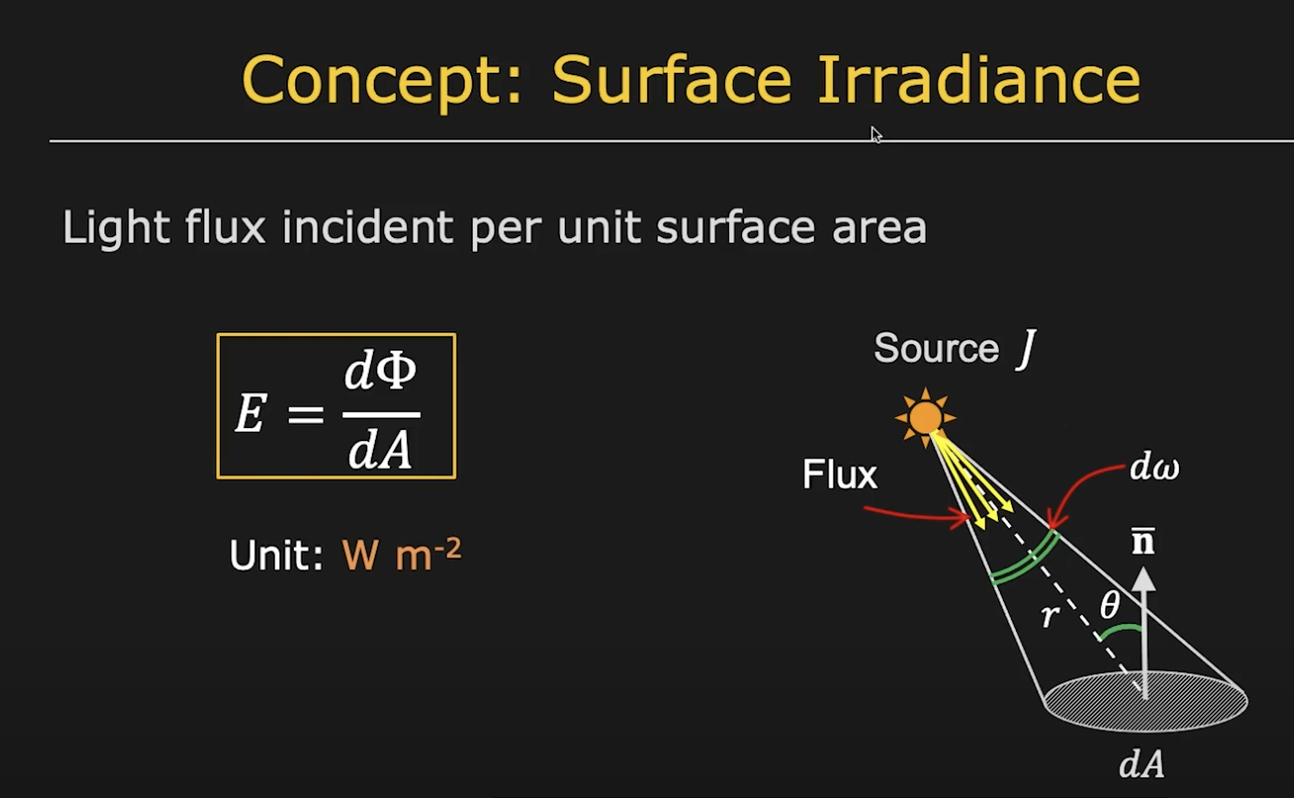
\includegraphics[width=5cm]{00temppic/5.png}
                    % \caption{多重路徑傳輸\cite{pic:multipath}}
                    % \label{pic:multipath}
                \end{figure}
                每單位面積所含的通量稱為輻照度,其中照射面積隨著距離$D$增加而平方遞增,在已知距離的情況下,即可利用立體角的定義,換算輻射強度與輻照度之間的關係\ref{eqn:I2E},$\omega$為入射表面與光源之夾角。
                
                \begin{equation}
                    \label{eqn:I2E}
                    E=I\cos\omega/D^2
                \end{equation}

                
             
        \end{description}

        

        

    \subsection{LED與PD的硬體參數與特性}
        \subsubsection{擺放自由度}
        LED與PD硬體有許多種類,最常見的市面上LED與PD為軸對稱並滿足朗博輻射模式(Lambertian Radiation Pattern),本論文僅考慮此類硬體。軸對稱代表當LED或PD僅對出射角或入射角以及距離有敏感度,以球座標系來看,凡在同一仰角與距離,無論方位角為何,光照強度與感光強度皆相同。

        因此,在描述座標系空間中的LED與PD時,一共有五個自由度,包含擺放位置$P$的三個分量$x,y,z$,以及定義指向的單位向量$N$。由於LED與PD皆為軸對稱,因此僅有兩個自由度:仰角$\alpha$與方位角$\beta$,$N$在卡氏座標系下的xyz分量則為$u,v,w$。

        %補公式

        \begin{figure}[ht]
            \centering
            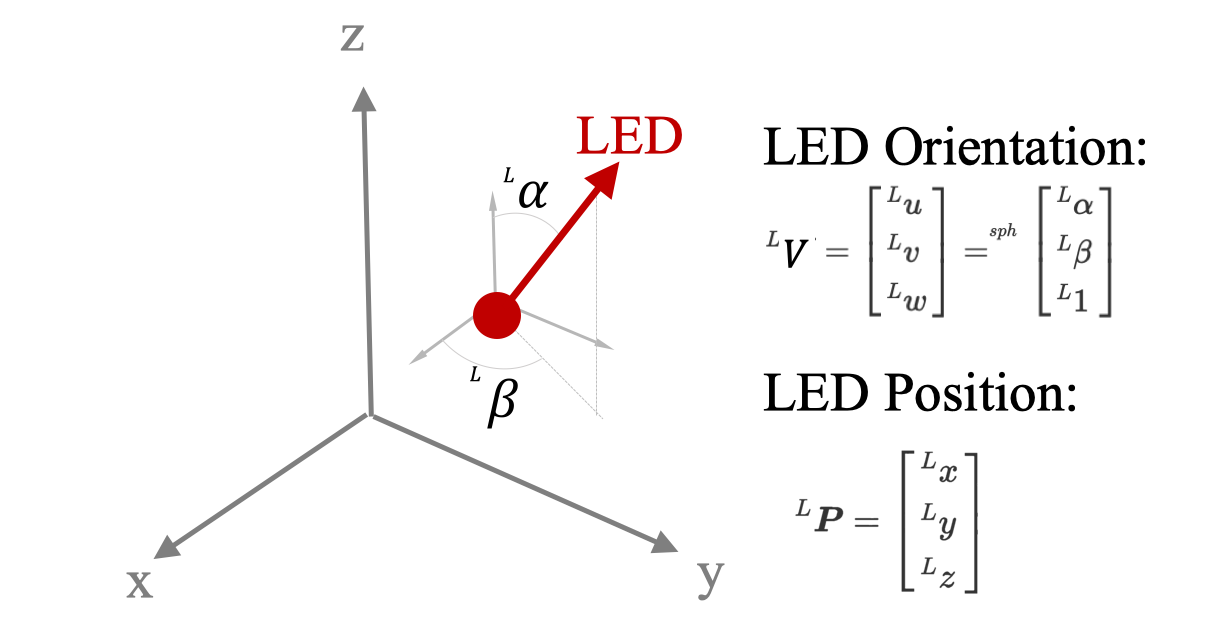
\includegraphics[width=10cm]{ch2pic/LED_config.png}
            \caption{LED在座標系中的擺放自由度}
            \label{pic:led_config}
        \end{figure}

        \subsubsection{朗博輻射模式}

        LED與PD的照射與接收模式(Pattern)可以用Lambertian Radiation Pattern量化,代表感光與發光強度隨著LED出射角與PD入射角的增加而變小,其衰減模式可用餘弦函數(cosine)的M次方(power)表示,M代表的是Lambertian Order。

        以二維的角度來看如圖,LED光照射的能量隨出射角度增加而減少,在LED中心軸的方向強度最高,在此描述LED強度時不考慮距離。如先前所述,LED為軸對稱,因此三維的照射模式即為二維模式以中心軸旋轉。在同樣出射角下,光輻射強度相同。
        
        有了光輻射強度在不同入射角的關係,將整個半球中的輻射強度積分,得到LED在整個半球上所照射的總瓦數比例,將該值倒數,即可由LED發射之總能量推算各入射角的光輻射強度。

        \begin{equation}
            I(\omega)=I(\omega=0)\times\cos(\omega)^{M}\\
            I(\omega)=Pt\frac{(M+1)}{2 \pi} \cos \omega^{M}
        \end{equation}

        \subsubsection{硬體參數}

        \begin{figure}[ht]
            \caption{LED與PD對模式與強度影響之硬體參數}
            \label{tab:hardwarepara}
            \centering
            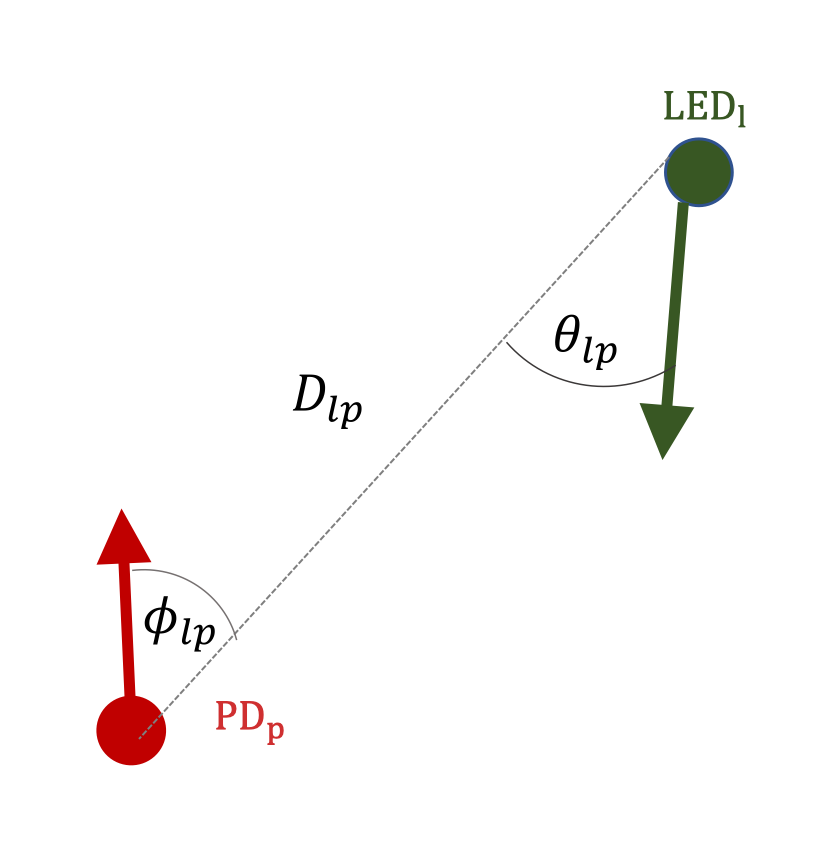
\includegraphics[width=6cm]{00temppic/7.png}
        \end{figure}

        % 實際硬體挑選時所需注意的參數
        

    \subsection{光傳遞模型}
    
    \begin{figure}[ht]
        \caption{LED與PD的交互關係}
        % \label{tab:hardwarepara}
        \centering
        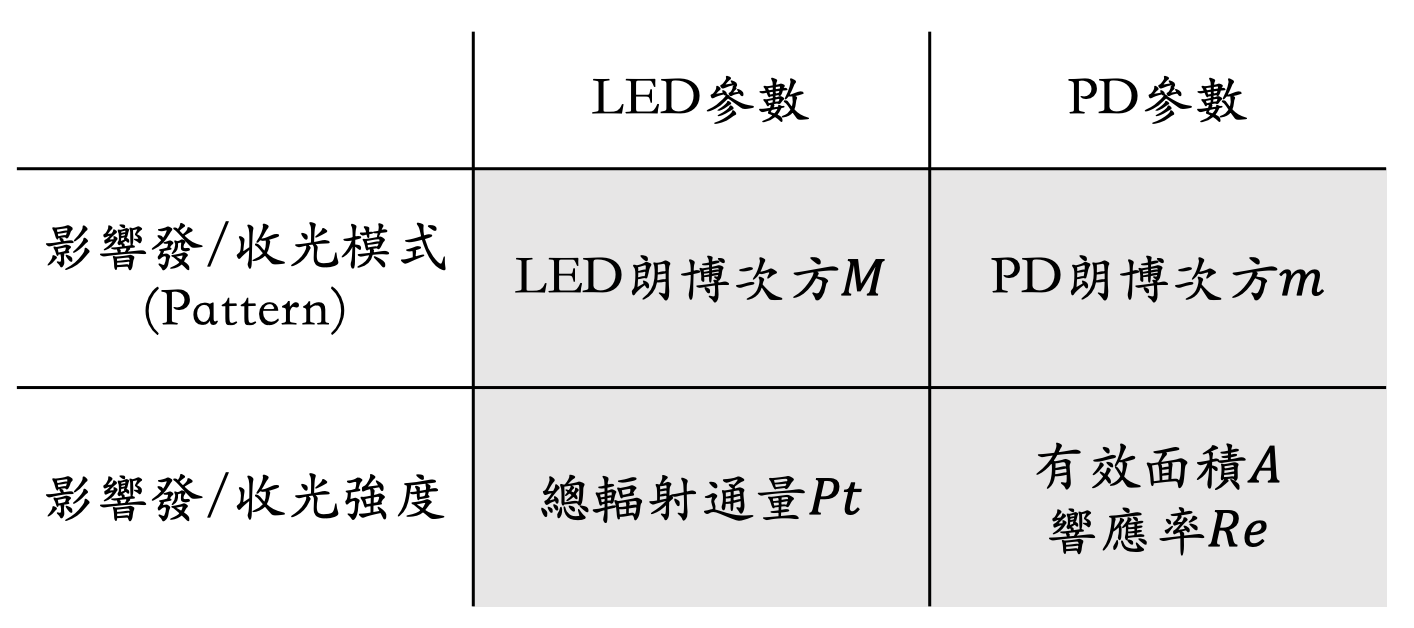
\includegraphics[width=6cm]{ch2pic/tab_hardwarepara.png}
    \end{figure}

    第$p$個LED量測到第$l$個LED的強度$\Phi_{lp}$可由\ref{eqn:model}描述。
    
    \begin{equation}
        \label{eqn:model}
        \Phi_{lp}=\frac{ A_p\cos\phi_{lp}^{m_{p}} }{D^2_{lp}}\times Pt_l\frac{(M_{l}+1)}{2 \pi} \cos \theta_{lp}^{M_{l}}  \\
        =k_{lp}\frac{{\cos\theta_{lp}}^{M_{l}}{\cos\phi_{pl}}^{m_{p}}}{D_{lp}^2}\\
    \end{equation}

    
    
    

        
        
    %     討論完LED與角度的關係後,再來考慮光能量與距離的關係。考慮同一Solid angle下的一束光,隨傳遞距離拉長,所照射到的表面積增加,因此「能量」隨距離平方遞減。
        
    %     綜合角度與距離的影響,空間中任一點的「光大小」如式
        
    %     接著考慮PD接收的Model,PD的接收能量與入射角同樣遵守Lambertian Pattern,變數一樣包含入射角以及Lambertian Order。除了角度以外,藉由乘上PD的硬體參數感光面積得到該PD所感測到的瓦數,PD會將感受到的光瓦數轉換為電流輸出,其中轉換比例為Responsivity。
        
    %     舉具體的例子來描述lambertian order的影響,M越大的LED,光強度隨出射角度衰減的速度越大,而照射範圍則越小。在挑選硬體時,M的選擇則為強度與範圍的取捨。同樣總輻射能量的LED,不同M隨角度的發光強度如圖示,首先可以觀察到M越小所覆蓋的角度範圍越大,而中心軸的光強度也小很多,其原因是因為其照射範圍大,因此在半球面上大角度的積分,入射角度越大時在半球面上的面積越大。
        
    %     從硬體層面來看,LED與PD的照射範圍


        



    \subsection{LED與PD定位系統}

        LED與PD的相對定位量測系統中,根據\ref{chp:relative}目標物為LED座標系,剛體上裝載著主動發送訊號的LED;而量測者為PD座標系,上面裝載著傳感器收取資訊;兩座標系上的感測器與訊號發送器皆為固定的,可以想像成將PD焊於電路板上,封裝成一量測儀器,並以螺絲等固定在量測者剛體上,隨著量測者與目標物移動時,兩座標系之間的座標轉換關係會改變,然而PD與其座標轉換關係並不會改變,LED亦然。

        %補
        [覺得應該要補硬體怎麼編碼解碼的]



    \subsection{LED與PD定位文獻探討}

        了解LED與PD定位系統的運作方式後,本章節介紹現有文獻的成果,並舉實例情境來凸顯此領域不足之處,提出可改善之方向。
        
        (不確定走向,所以先用列表整理在Notion之後確定再補上)
        % 補

        \begin{figure}[ht]
            \centering
            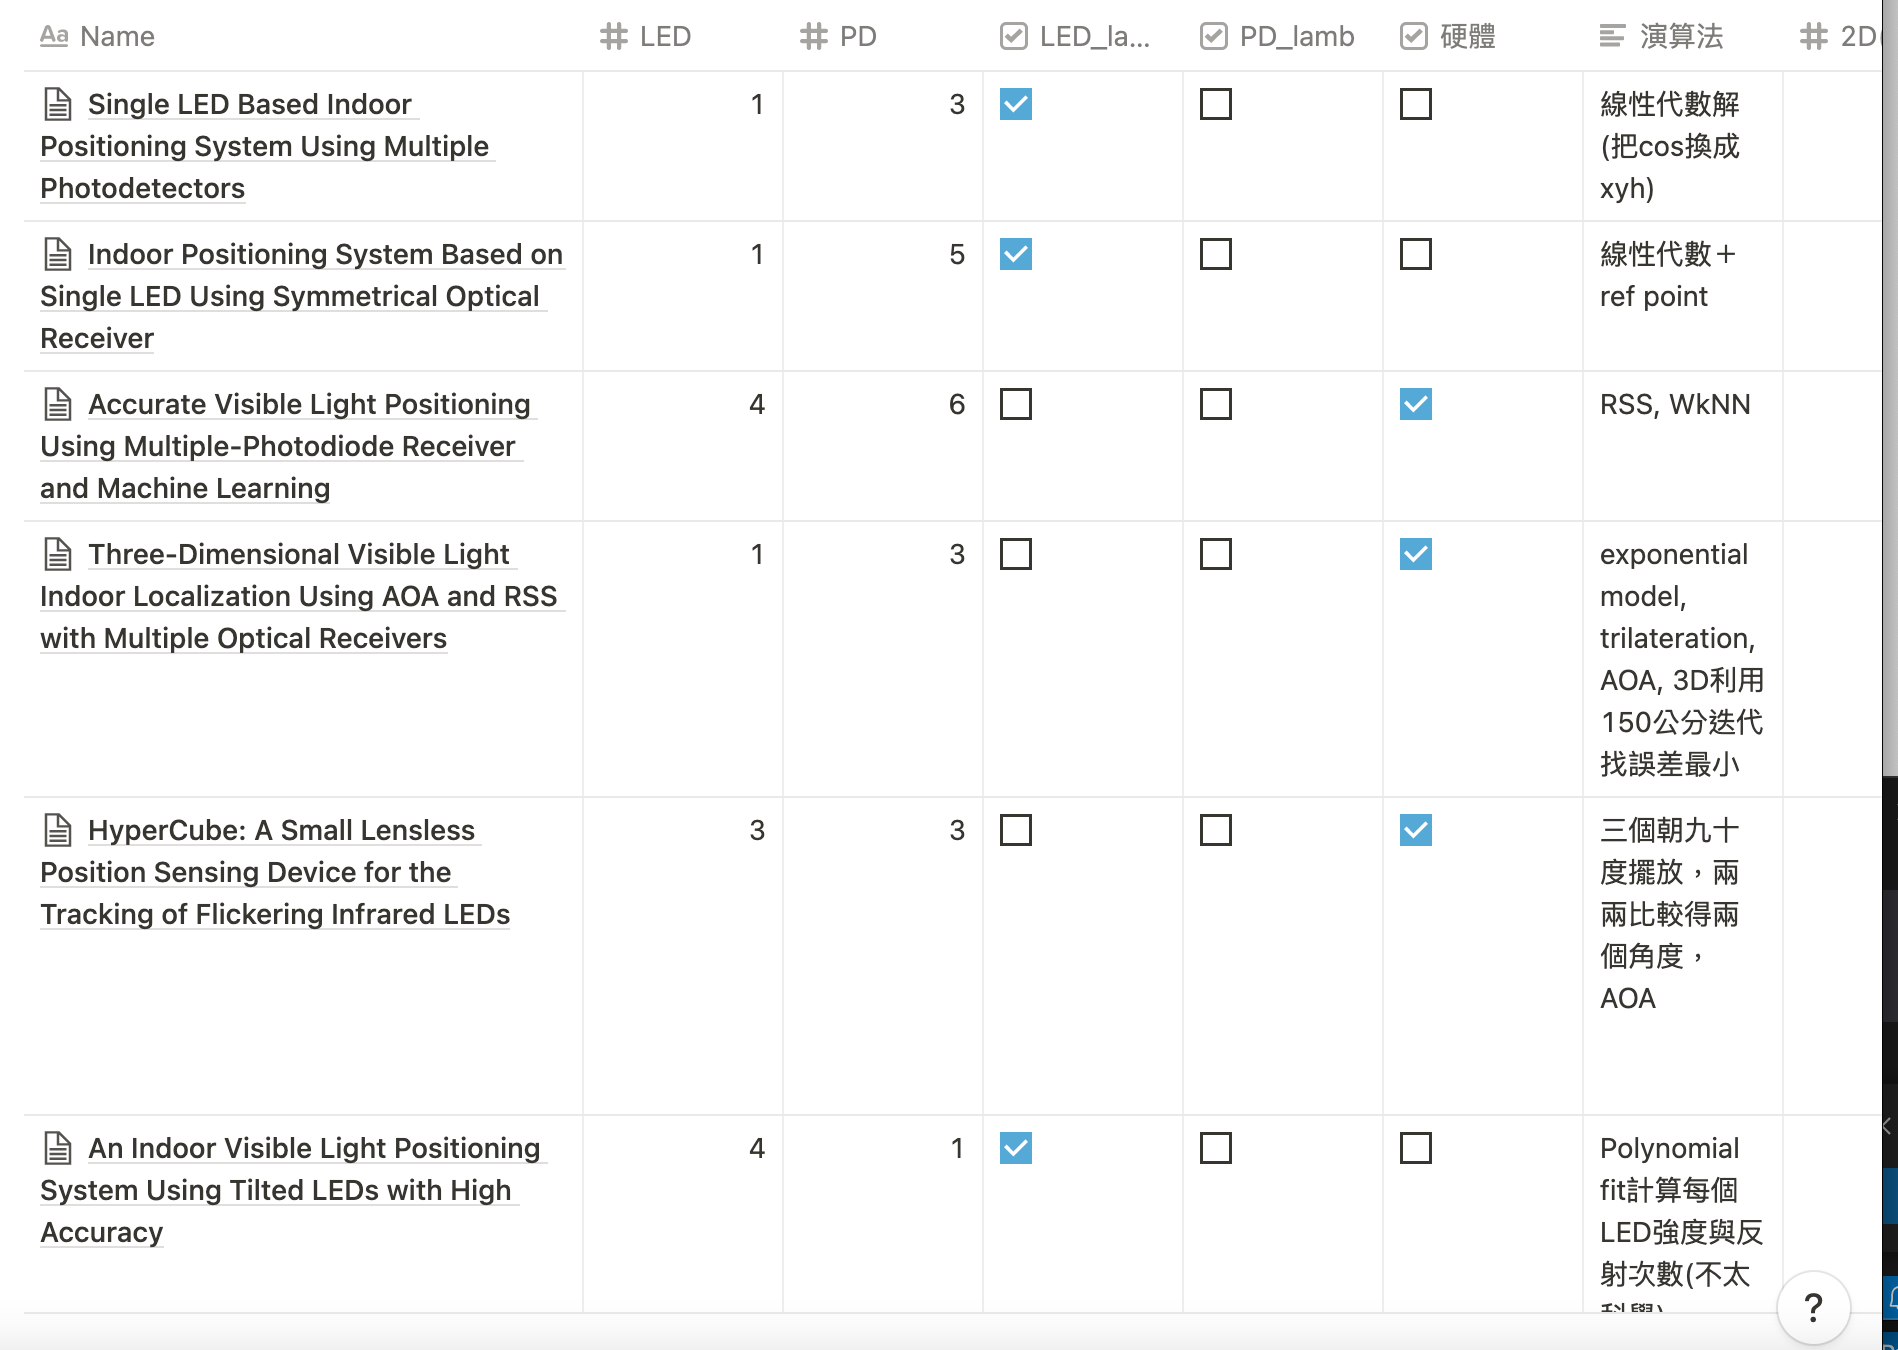
\includegraphics[width=10cm]{00temppic/temp.png}
            % \caption{多重路徑傳輸\cite{pic:multipath}}
            % \label{pic:multipath}
        \end{figure}



\section{結論}

雖然此種做法已被討論且有潛力,但缺少完整考慮[三維、組態、硬體參數]的方式,因此本論文有以下研究成果:
\begin{itemize}
    \item 利用LED與PD進行三維相對位置量測的方法,於第三章詳述。
    \item 為了將第三章所提出之相對位置量測方法,靈活應用於不同情境,提出針對不同使用情境的最佳化方法,藉由調整硬體參數、LED與PD的組態(Deployment),改善系統表現,於第四章詳述。
    \item 第五章將提出之最佳化方法實作,以不同情境做為模擬案例,為各自設計最佳的量測系統參數與組態,並進行分析與比較。
    \item 第六章針對本論文的研究成果總結,並提出未來改善方向。
\end{itemize}